\documentclass{article}
\usepackage[utf8]{inputenc}

\usepackage{amssymb}
\usepackage{amsmath}
\usepackage{float}
\usepackage[toc,page]{appendix}
\usepackage{listings}
\usepackage{geometry}
\geometry{
a4paper,
top=1in
}

\DeclareMathOperator{\Var}{Var}
\DeclareMathOperator{\Corr}{Corr}
\DeclareMathOperator{\Cov}{Cov}

\title{Time Series Project 2}
\author{Stefan Eng and Franz Hartleitner}
\date{May 2019}

\usepackage{natbib}
\usepackage{graphicx}

\begin{document}

\maketitle

\section*{Problem 1}

\begin{figure}[H]
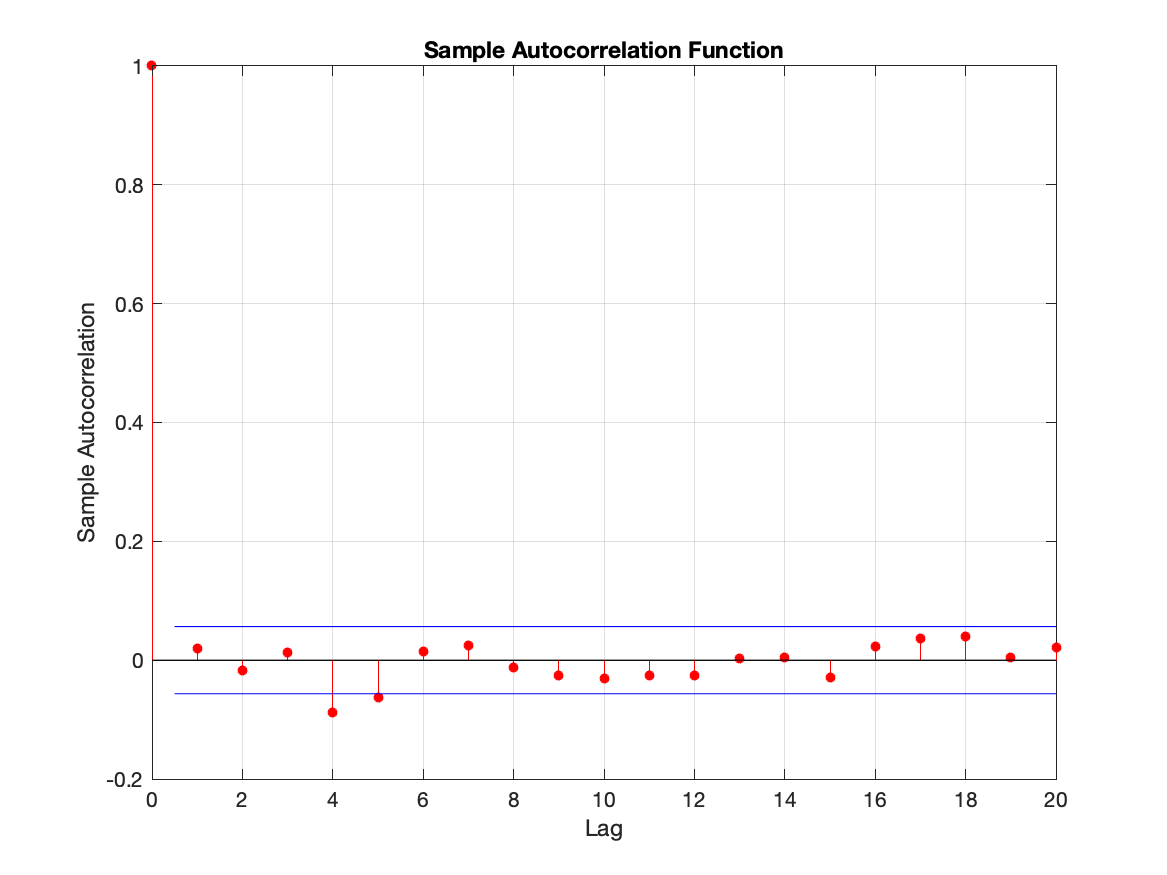
\includegraphics[width=10cm]{plots/acf_log_rtns.png}
\centering
\caption{Autocorrelation function for the log returns}
\label{fig:acf_log_rtns}
\end{figure}

\begin{figure}[H]
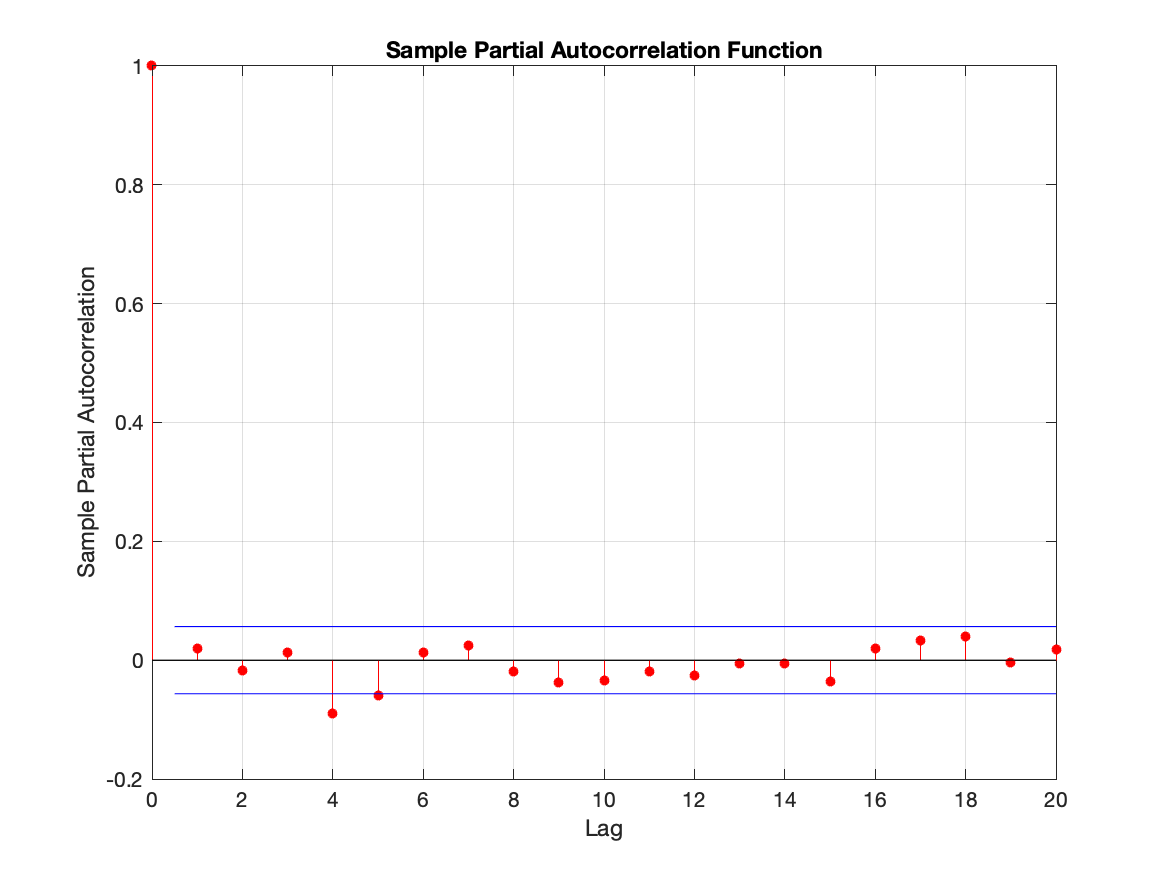
\includegraphics[width=10cm]{plots/pacf_log_rtns.png}
\centering
\caption{Partial autocorrelation function for the log returns}
\label{fig:pacf_log_rtns}
\end{figure}

\section*{Problem 2}

\begin{figure}[H]
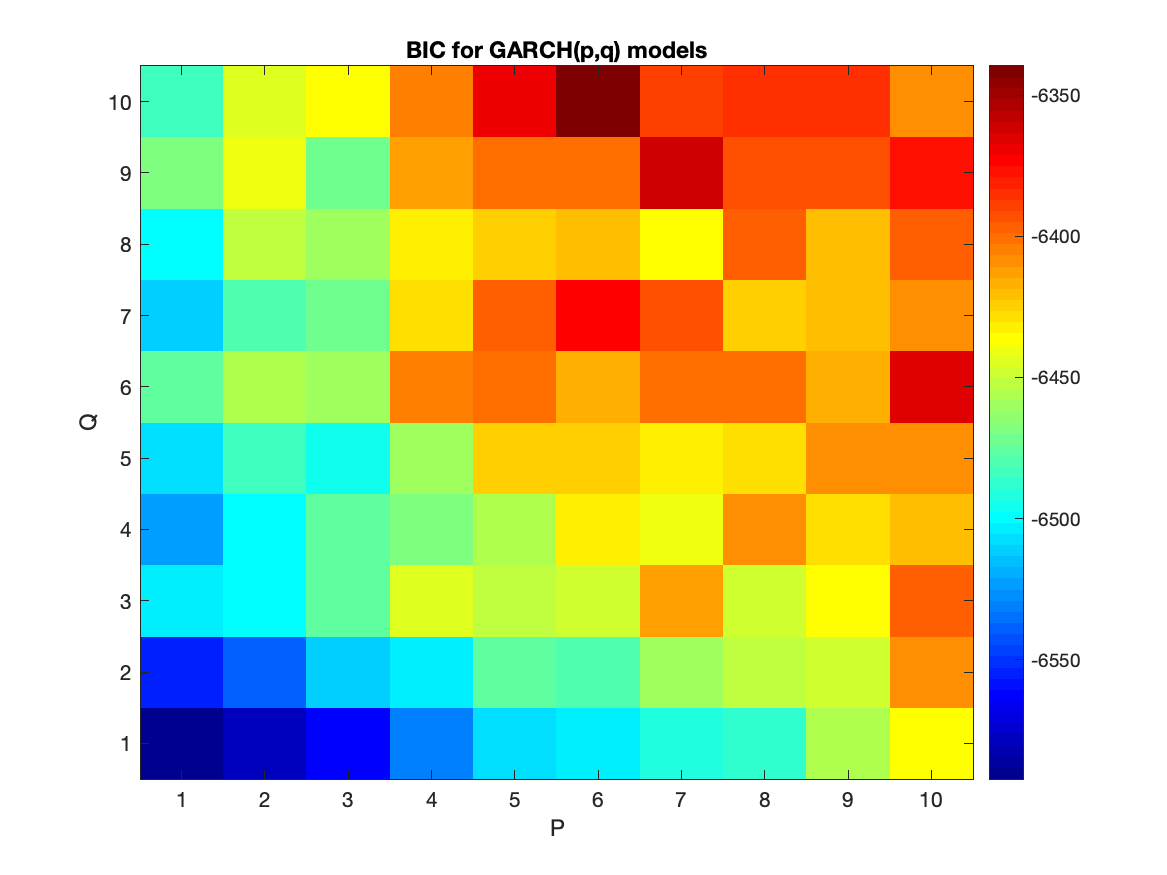
\includegraphics[width=10cm]{plots/bic_heatmap_norm.png}
\centering
\caption{BIC Heatmap for GARCH(p,q) process with Gaussian noise}
\label{fig:bic_heatmap_norm}
\end{figure}

\section*{Problem 3}

\begin{figure}[H]
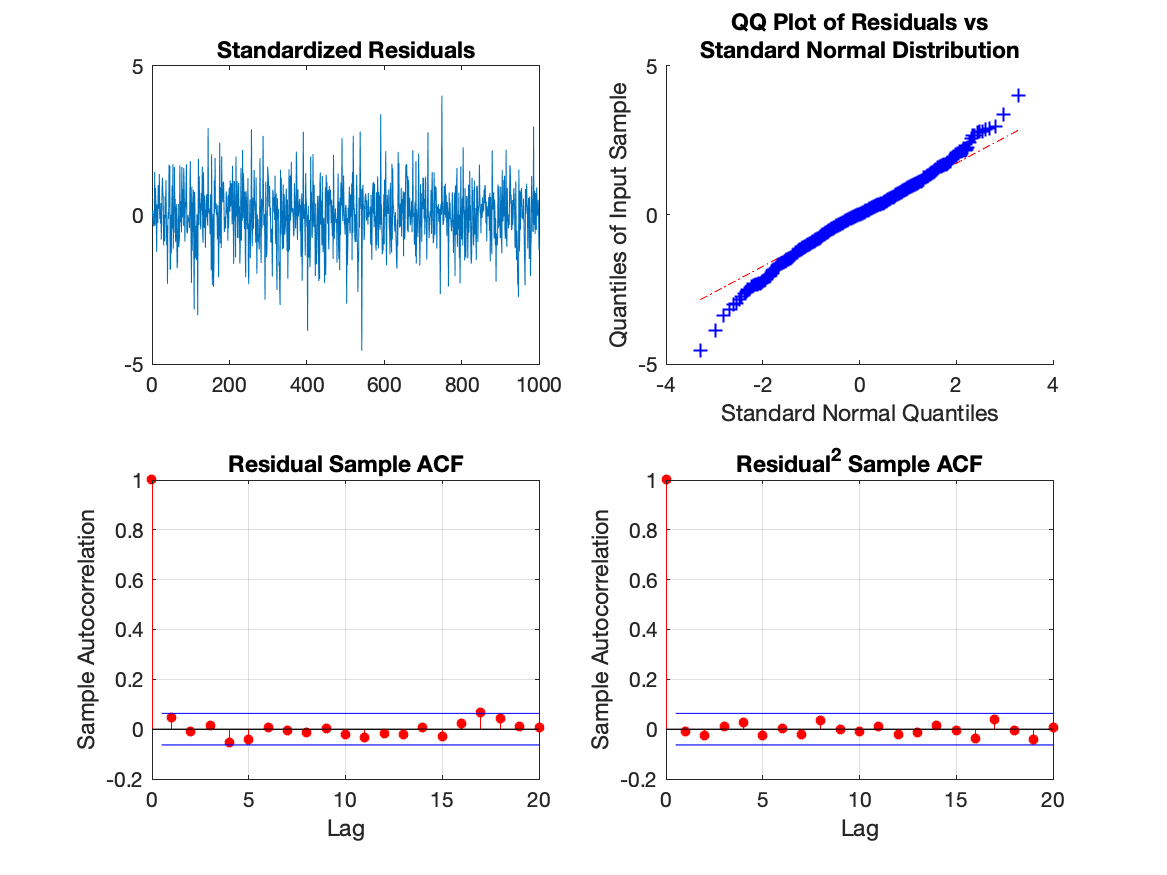
\includegraphics[width=10cm]{plots/residual_plots_norm.png}
\centering
\caption{Residual Plots for GARCH(1,1) process with Gaussian noise}
\label{fig:residual_plots_norm}
\end{figure}

\section*{Problem 4}

\begin{figure}[H]
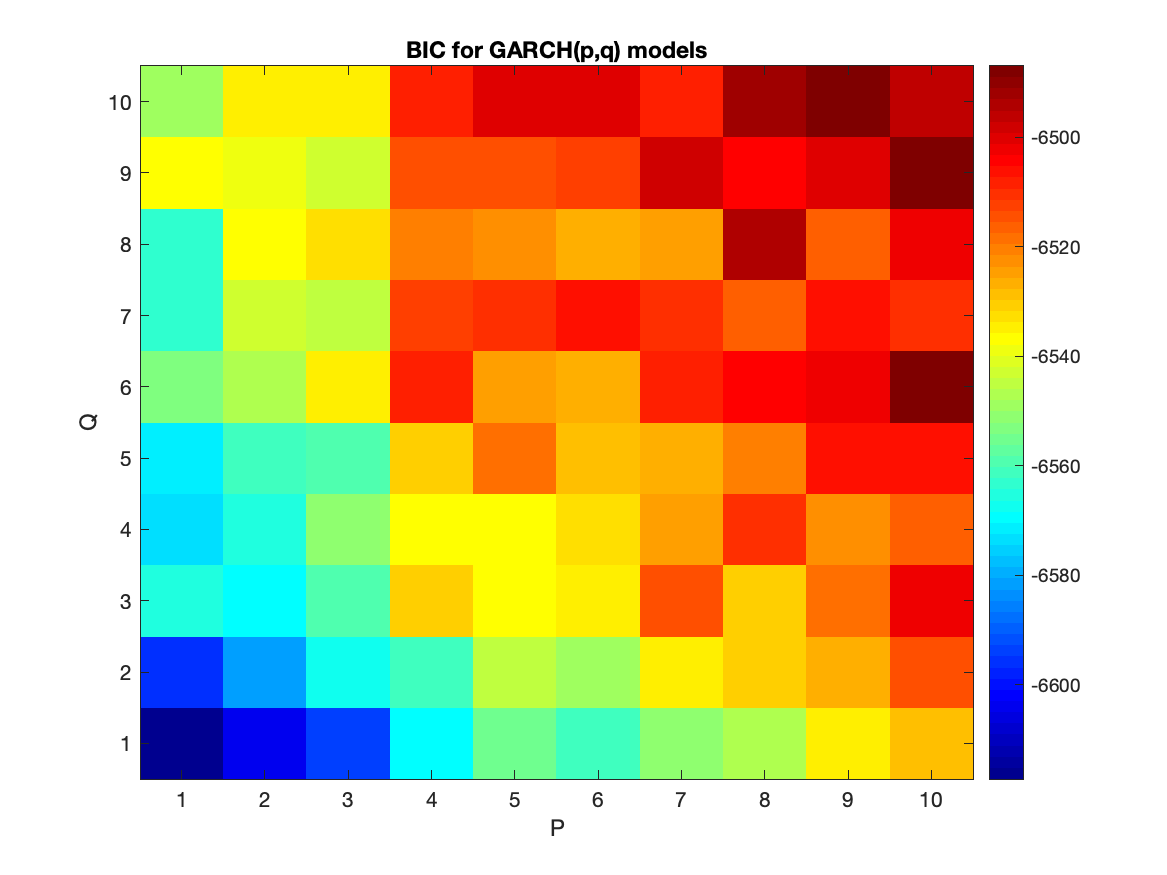
\includegraphics[width=10cm]{plots/bic_heatmap_t.png}
\centering
\caption{BIC Heatmap for GARCH(p,q) process with Student's t distribution noise}
\label{fig:bic_heatmap_norm}
\end{figure}

\begin{figure}[H]
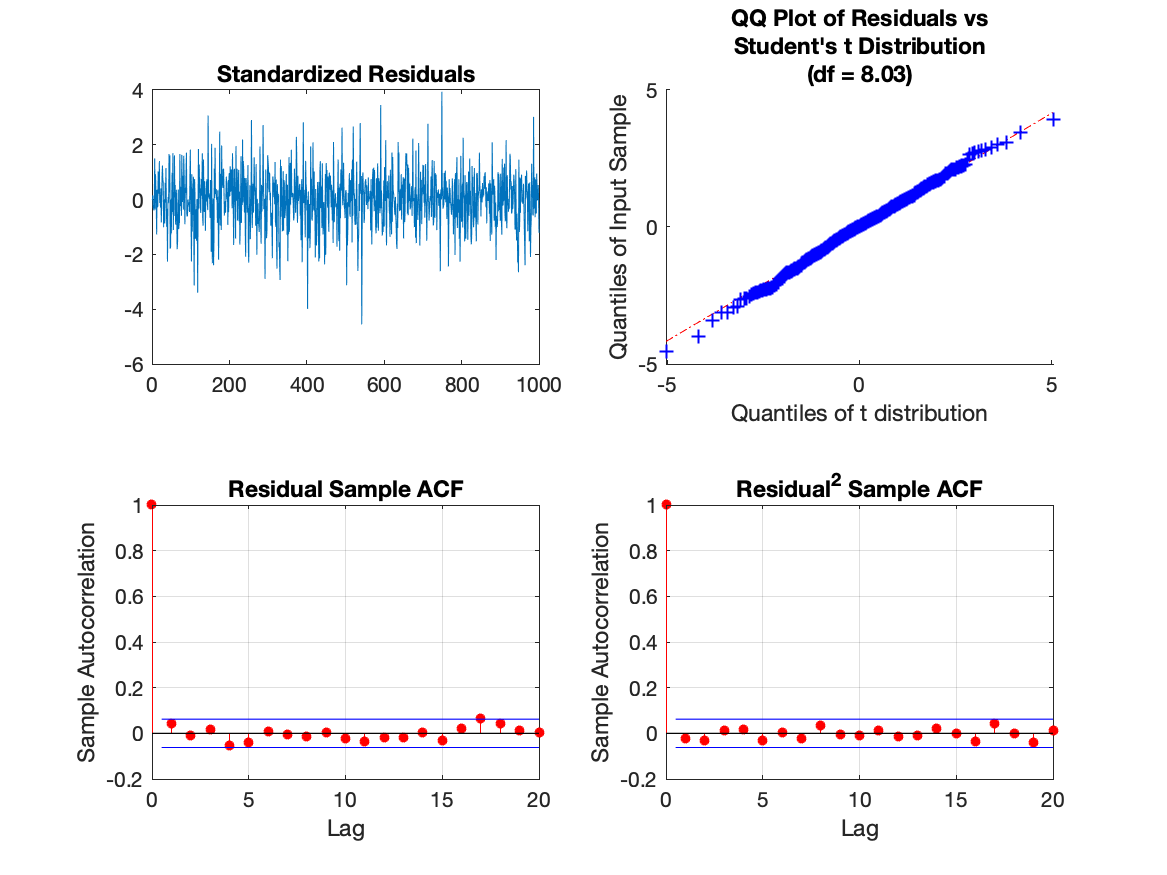
\includegraphics[width=10cm]{plots/residual_plots_t.png}
\centering
\caption{Residual Plots for GARCH(1,1) process with Student's t distribution noise}
\label{fig:residual_plots_norm}
\end{figure}

\begin{appendices}

\subsection{project1.m}
\lstinputlisting[language=Octave]{project2.m}

\end{appendices}

%\bibliographystyle{plain}
%\bibliography{references}
\end{document}
